\documentclass[a4paper,14pt]{article}

\usepackage{comment} % Para comentar várias linhas ao mesmo tempo

%matemática
\usepackage{amsmath}
\usepackage{amssymb}

%diagramação
\usepackage{extsizes}
\everymath{\displaystyle}
\usepackage{geometry}
\usepackage{fancyhdr}
\usepackage{multicol}
\usepackage{graphicx}
\usepackage[brazil]{babel}
\usepackage[shortlabels]{enumitem}
\usepackage{cancel}
\usepackage{textcomp}
\usepackage{tcolorbox}

%tabelas
\usepackage{array} % Para melhor formatação de tabelas
\usepackage{longtable}
\usepackage{booktabs}  % Para linhas horizontais mais bonitas
\usepackage{float}   % Para usar o modificador [H]
\usepackage{caption} % Para usar legendas em tabelas
\usepackage{wrapfig} % Para usar tabelas e figuras flutuantes
\usepackage{xcolor} % Para cores do fundo de tabelas
\usepackage{colortbl} % Para cores do fundo de tabelas

%tikzpicture
\begin{comment}
	\usepackage{tikz}
	\usepackage{scalerel}
	\usepackage{pict2e}
	\usepackage{tkz-euclide}
	\usetikzlibrary{calc}
	\usetikzlibrary{patterns,arrows.meta}
	\usetikzlibrary{shadows}
	\usetikzlibrary{external}
\end{comment}


%pgfplots
\usepackage{pgfplots}
\pgfplotsset{compat=newest}
\usepgfplotslibrary{statistics}
\usepgfplotslibrary{fillbetween}

%colours
\usepackage{xcolor}



\columnsep=2cm
\hoffset=0cm
\textwidth=8cm
\setlength{\columnseprule}{.1pt}
\setlength{\columnsep}{2cm}
\renewcommand{\headrulewidth}{0pt}
\geometry{top=1in, bottom=1in, left=0.7in, right=0.5in}

\pagestyle{fancy}
\fancyhf{}
\fancyfoot[C]{\thepage}

\begin{document}
	
	\noindent\textbf{6FMA109 - Matemática} 
	
	\begin{center}Exercícios (I) (Versão estudante)
	\end{center}
	
	\noindent\textbf{Nome:} \underline{\hspace{10cm}}
	\noindent\textbf{Data:} \underline{\hspace{4cm}}
	
	%\section*{Questões de Matemática}
	
	\begin{multicols}{2}
		\begin{enumerate} 
			\item O triângulo $A'B'C'$ da figura a seguir é congruente ao triângulo $ABC$. Calcule as medidas de $x, y$ e $z$. \\
			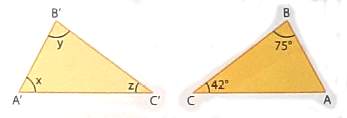
\includegraphics[width=1.1\linewidth]{6FMA109_imagens/imagem1}
			\\\\\\\\\\\\\\\\\\\\
			\item  Na figura a seguir, $\Delta$$AMB \cong \Delta$$AMC$ e $m(A\hat{M}B) = $~90°. Sabendo que $m(A\hat{B}m) = $15°, qual é o valor de $m(B\hat{A}C)$? \\
				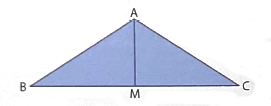
\includegraphics[width=1.1\linewidth]{6FMA109_imagens/imagem2}
				\\\\\\\\\\\\\\
			\item Dizer quais são as congruências na figura a seguir.
			\\
			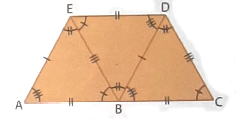
\includegraphics[width=1.1\linewidth]{6FMA109_imagens/imagem3}
			\\\\\\\\\\\\\\\\\\
			\item Calcule $BC$ na figura a seguir. \\
			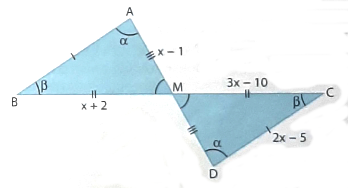
\includegraphics[width=1.1\linewidth]{6FMA109_imagens/imagem4}
			\\\\\\\\\\\\\\\\\\
			%81 a 83
			\item \begin{enumerate}[a)]
				\item Sabendo-se que $\Delta$$AMB \cong \Delta$$CMD$, calcule $x, y, z, a$ e $b$ na figura. \\
				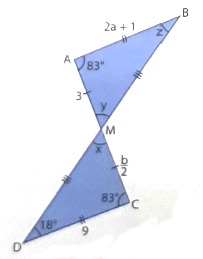
\includegraphics[width=1.1\linewidth]{6FMA109_imagens/imagem5} \\\\\\\\\\\\\\\\\\\\
			\end{enumerate}
			\item Determine os valores de $a$ e $b$ para que os triângulos $ABD$ e $CDB$ sejam congruentes e calcule o perímetro do quadrilátero $ABCD$ \\
			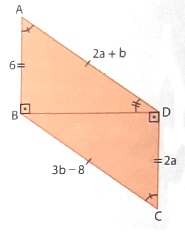
\includegraphics[width=1.1\linewidth]{6FMA109_imagens/imagem6}
			\\\\\\\\\\\\\\
			\item Na figura a seguir, os triângulos $ABC$ e $AED$ são congruentes entre si e $m(A\hat{B}C) = 30$°. Se o triângulo $ACD$ tem $m(C\hat{A}D) = m(A\hat{D}C) = m(D\hat{C}A) = 60$° e $AD = DC = CA = 4 $cm, calcule $\overline{BE}$ e $m(B\hat{A}E)$ \\
			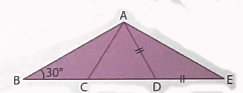
\includegraphics[width=1.1\linewidth]{6FMA109_imagens/imagem7}
		\end{enumerate}
		
		$~$ \\ 	$~$ \\ 	$~$ \\ 	$~$ \\ 	$~$ 
	\end{multicols}
\end{document}